%!TEX root = ../thesis.tex
\chapter{Results}
\label{Results}

In this section, we detail the findings of our experiments, where we tested the impact of each of the features on the outcome of the Bandit algorithm, on the same batches.  The features were Action Centering, Feedback Controller, Probability Clipping, Full vs Small Contextual feature set, which are abbreviated ac, fc, pc, small, respectively.  The name of each variant contains just the abbreviated feature names that are in use, with the naked variant using none of the features called No Features, and the full variant called ac fc pc.

Throughout the experiments, we compute the MUER using the same optimal probabilities of either $\pi_\text{min} = 0.1, \pi_\text{max} = 0.8$, even if probability clipping was not present or in the simple randomized treatment experiment; this is to allow for comparisons between different models using the same metrics.

Furthermore, using the optimization method using a standard deviation cutoff, as in algorithm \ref{Bandit Parameter Optimization, STD and Mean MUER}.


\section{Randomized Treatment}

As a baseline, we ran tests akin to the original HeartSteps v1 study, with purely random choices of action; we set this to be $\pi = 0.6$, but Figure \ref{RandomActionVsProbability} explores the relationship as $\pi$ varies between $[\pi_\text{min}, \pi_\text{max}]$ for each of the same $k=3$ CV training and testing batches we split into as the other experiments.  In general, the $MUER$ mean linearly increased or decreased depending on the set of users that were in the batch, and the $MUER$ standard deviation was convex, with an average minimum close to $0.55$.

\clearpage

\section{Impact of Bandit Features}

We investigate the utility of including each feature of the Bandit in this section, starting with a simple survey of the $MUER$ and continuing onto the Quality Metrics, depicted in Appendix \ref{Quality Metric Figures}.


\subsection{Overall $MUER$}

Below, we summarize statistics for $MUER$, with $N = 2500$ in each batch, for a total of $N = 7500$ in each averaged test.  We evaluate the quality of a bandit variant based on two axes: minimizing average $MUER$ and minimizing the total standard deviation of $MUER$.  The average $MUER$ measures the overall efficacy of the bandit variant, while the standard deviation of $MUER$ measures the fairness of treatment personalization.

In \ref{Boxplots of MUER for all Bandit Variants, sorted by mean MUER}, we note that while the mean $MUER$ does not favor more feature-laden bandit variants, we see that they serve well to reduce the variance, especially in the testing set.  The overall variance is minimized for variant ac fc pc, which is our full variant including action centering, feedback controlling, and probability clipping, while using the Full set of contextual features in the bandit model.  In the diagram, we also present the decomposition of total variance into within-user variance and between-user variance, discussed further in Section \ref{Variance Decomposition}.


In figure \ref{Cumulative Regrets for all Bandit Variants}, in particular for the full variant in dotted green, we see that the slope of the training cumulative regret starts off shallower than that of testing.  However, there is some concavity in the cumulative regret for the testing batches. Although the full variant has worse mean cumulative regret than most other variants at earlier time points, it evens out and is comparable to the others by the end.

One important note for figure \ref{Cumulative Regrets for all Bandit Variants} is that although the cumulative average $MUER$ appears to stop increasing for all variants and batches past decision point $175$, it does not.  Instead, it is due to the fact there were varying counts of data points for study participants, and past $175$, there were few left -- the flatness is due to the fact that their increasing cumulative regret is averaged out by the other users' cumulative regrets not increasing.

\begin{figure}[h!]
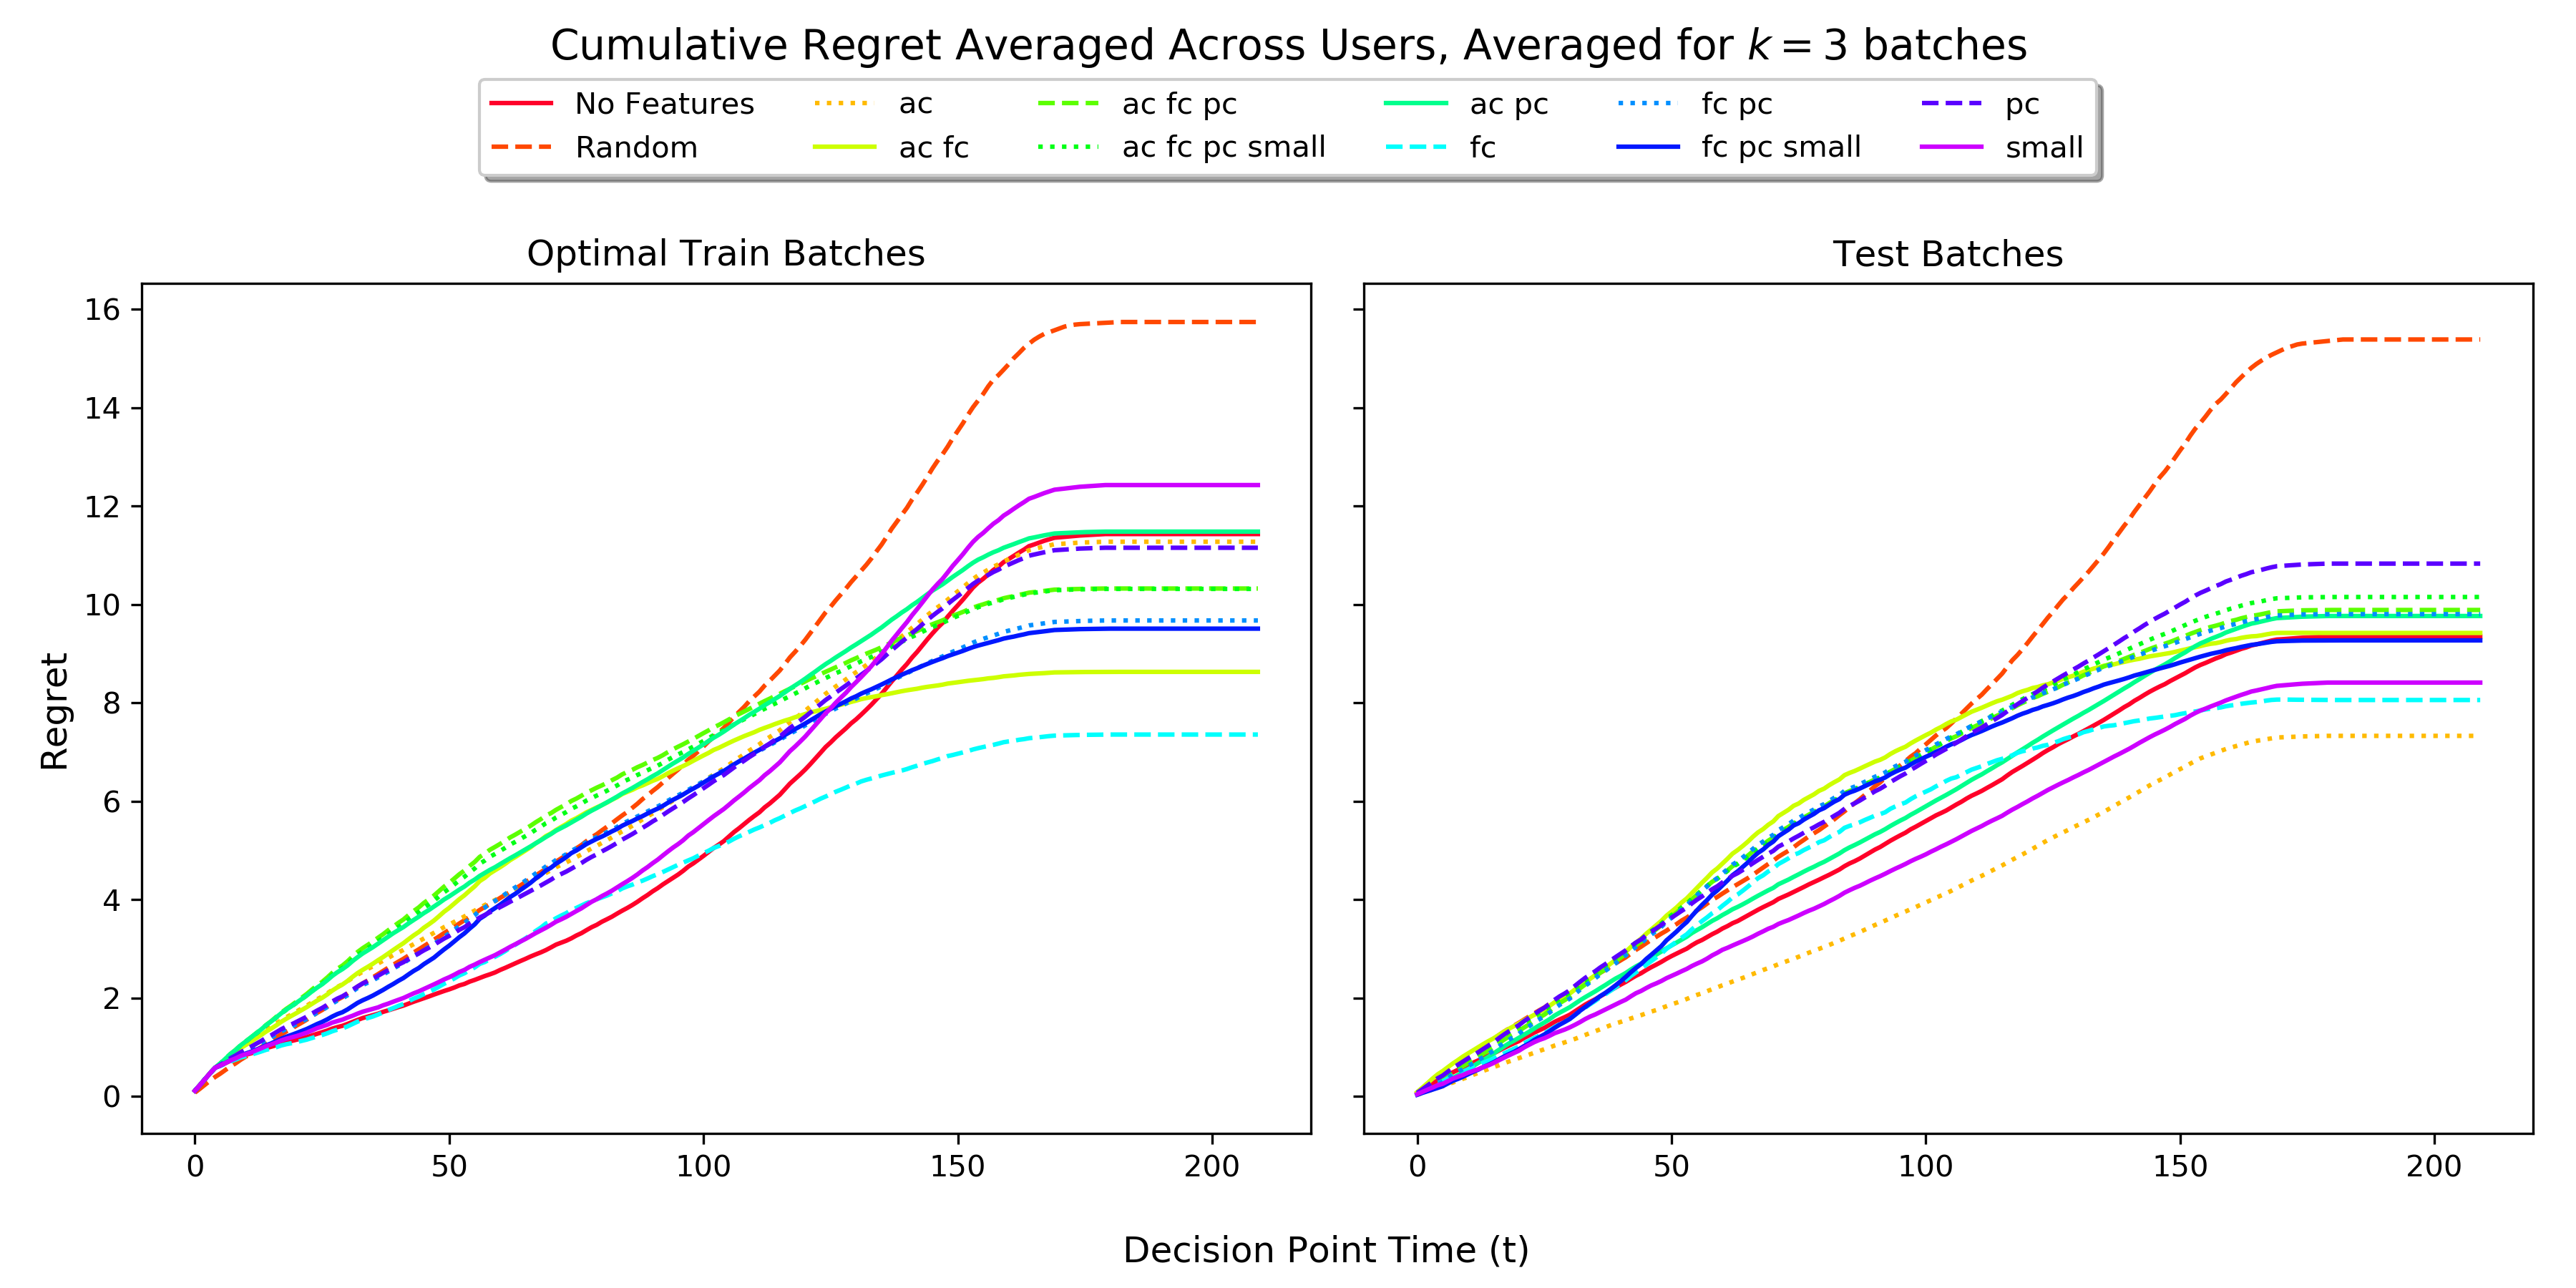
\includegraphics[width=1.3\textwidth,center]{figures/cum_regret_comparison_grouped.png}%
\caption{Cumulative regrets for all Bandit Variants, lower regret indicates better performance. (Separated Batches in Figure \ref{Cumulative Regrets for all Bandit Variants, Separated by Batch})}
\label{Cumulative Regrets for all Bandit Variants}
\end{figure}


\begin{figure}[H]
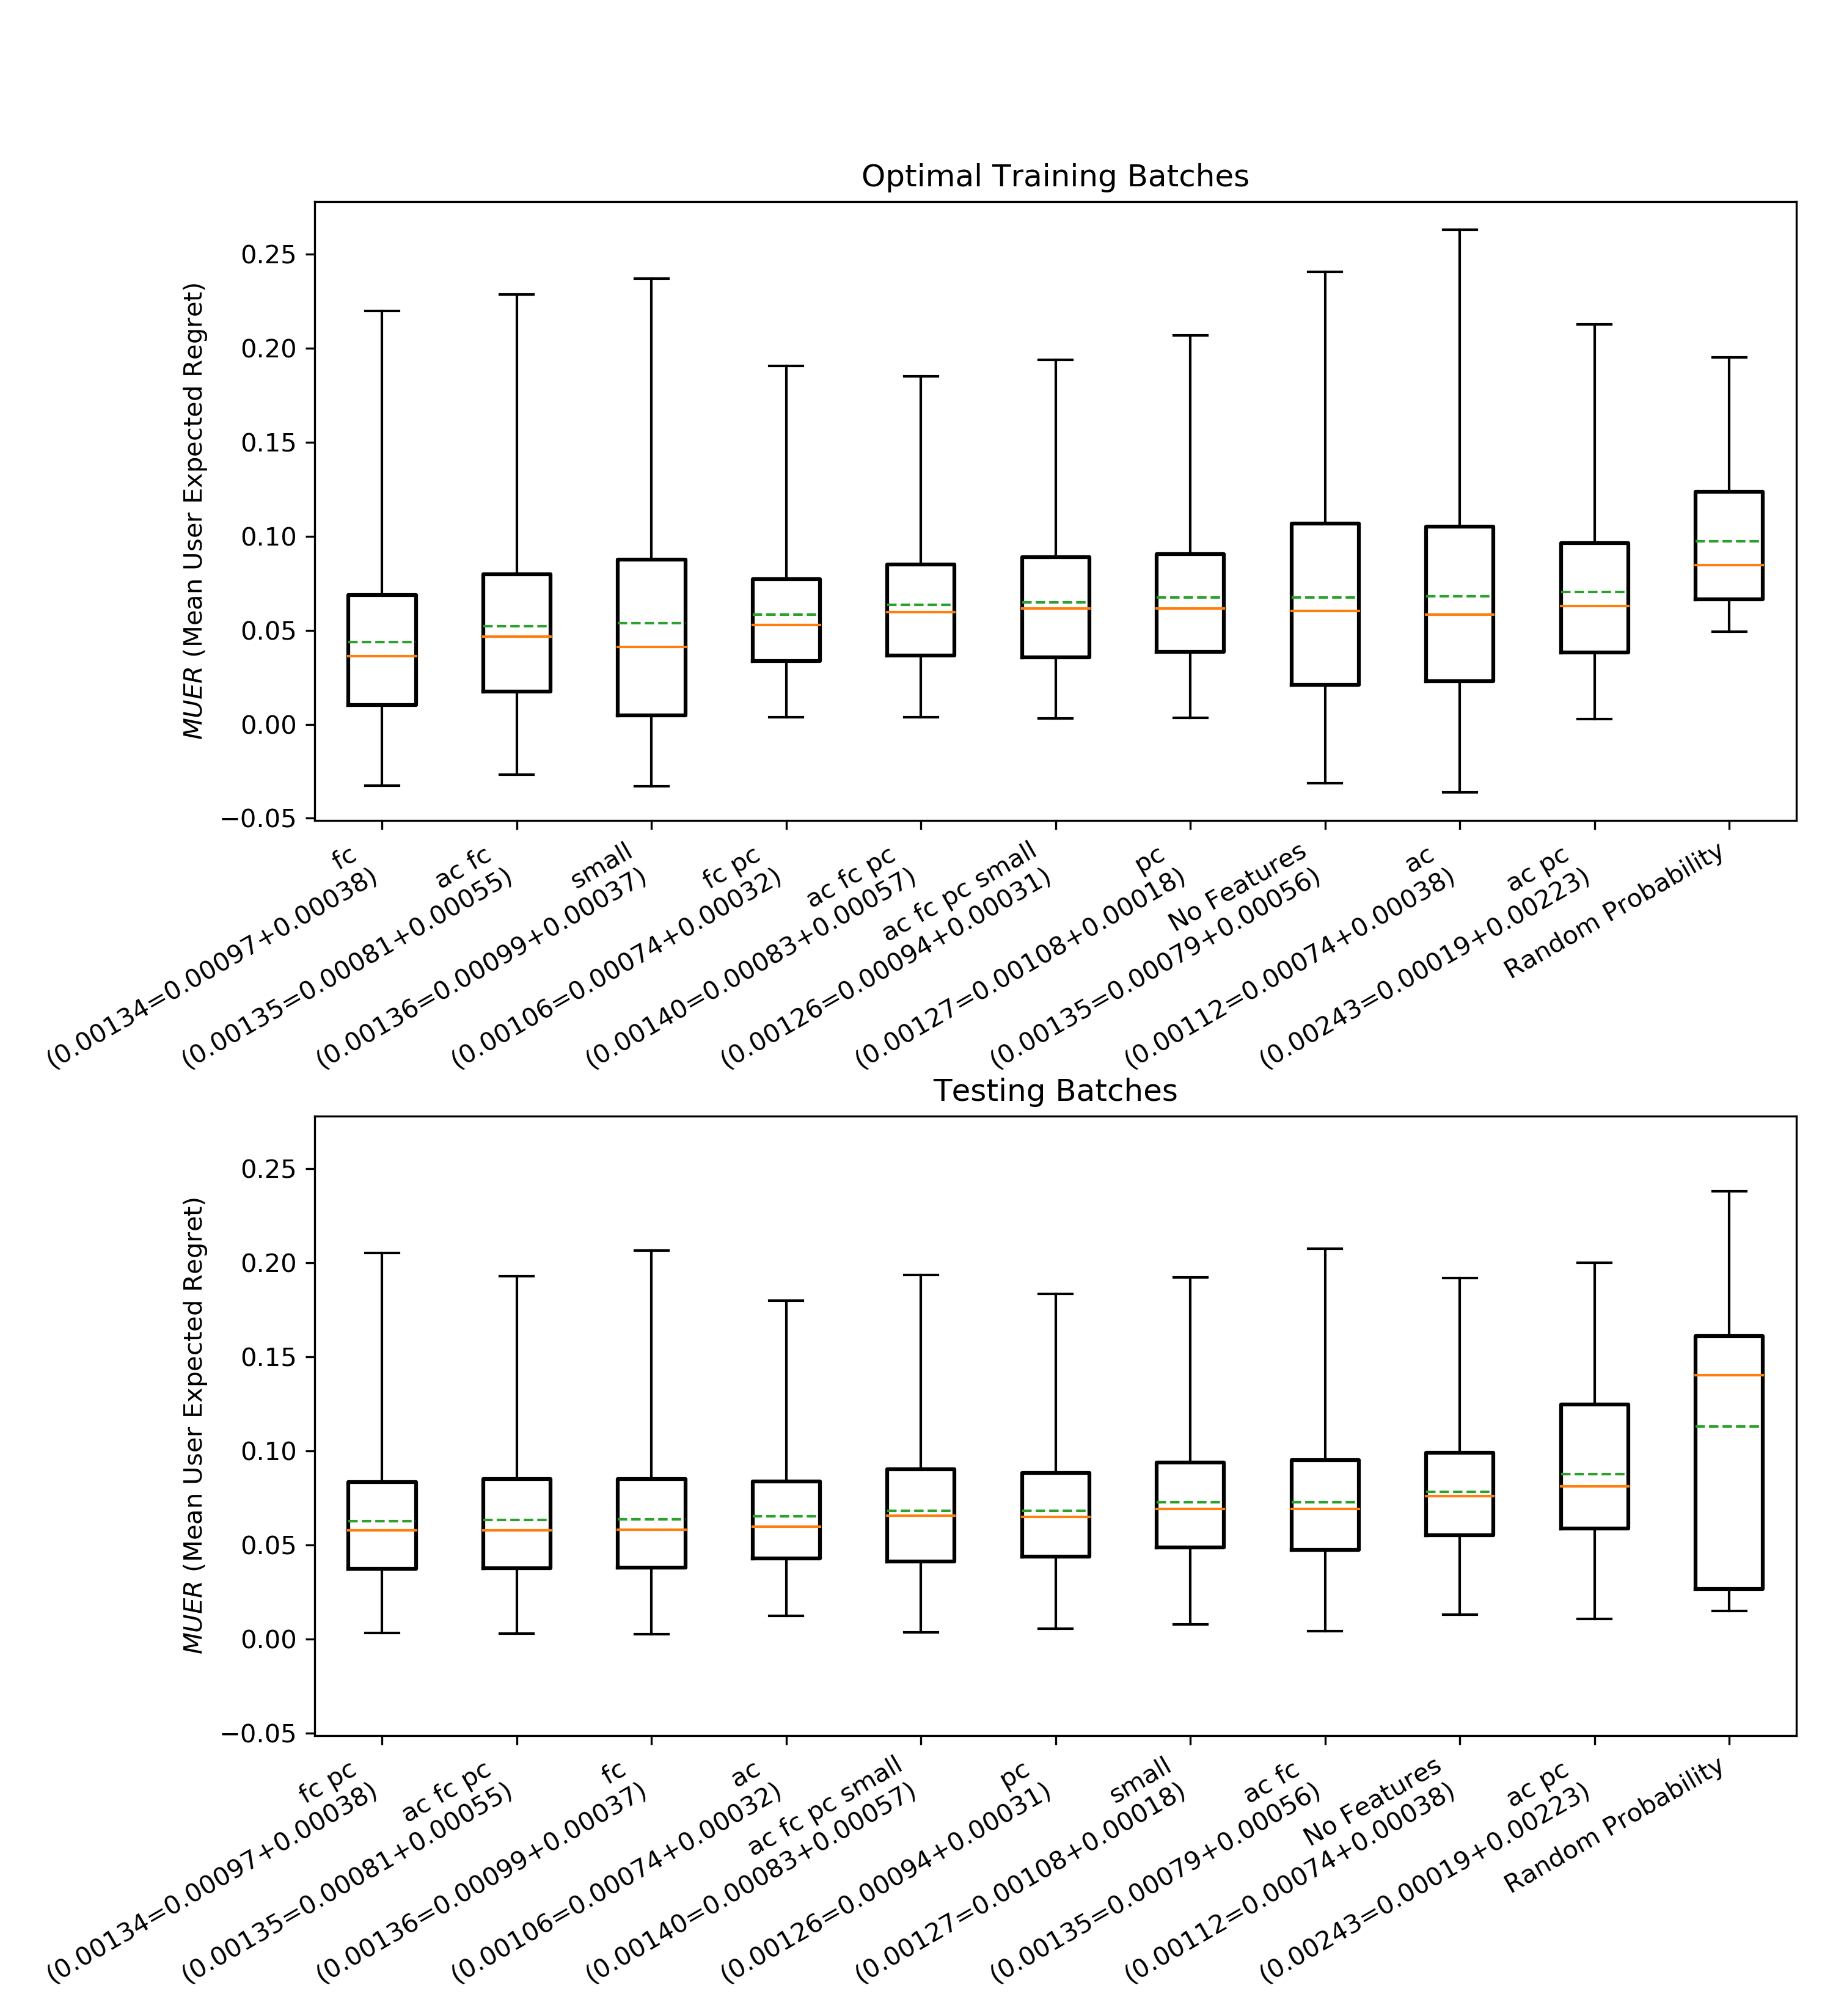
\includegraphics[width=1.25\textwidth,center]{figures/boxplots_muer.png}%
\caption{Boxplots of MUER for all Bandit Variants, sorted by mean $MUER$.  Mean in Green, Median in Orange.  Lower means and lower variance indicate better performance.  Variance Decomposition shown in label under each Variant name: $\langle\textit{Total Var}\rangle = \langle\textit{Within Var}\rangle + \langle\textit{Between Var}\rangle$}
\label{Boxplots of MUER for all Bandit Variants, sorted by mean MUER}
\end{figure}



\begin{figure}[H]
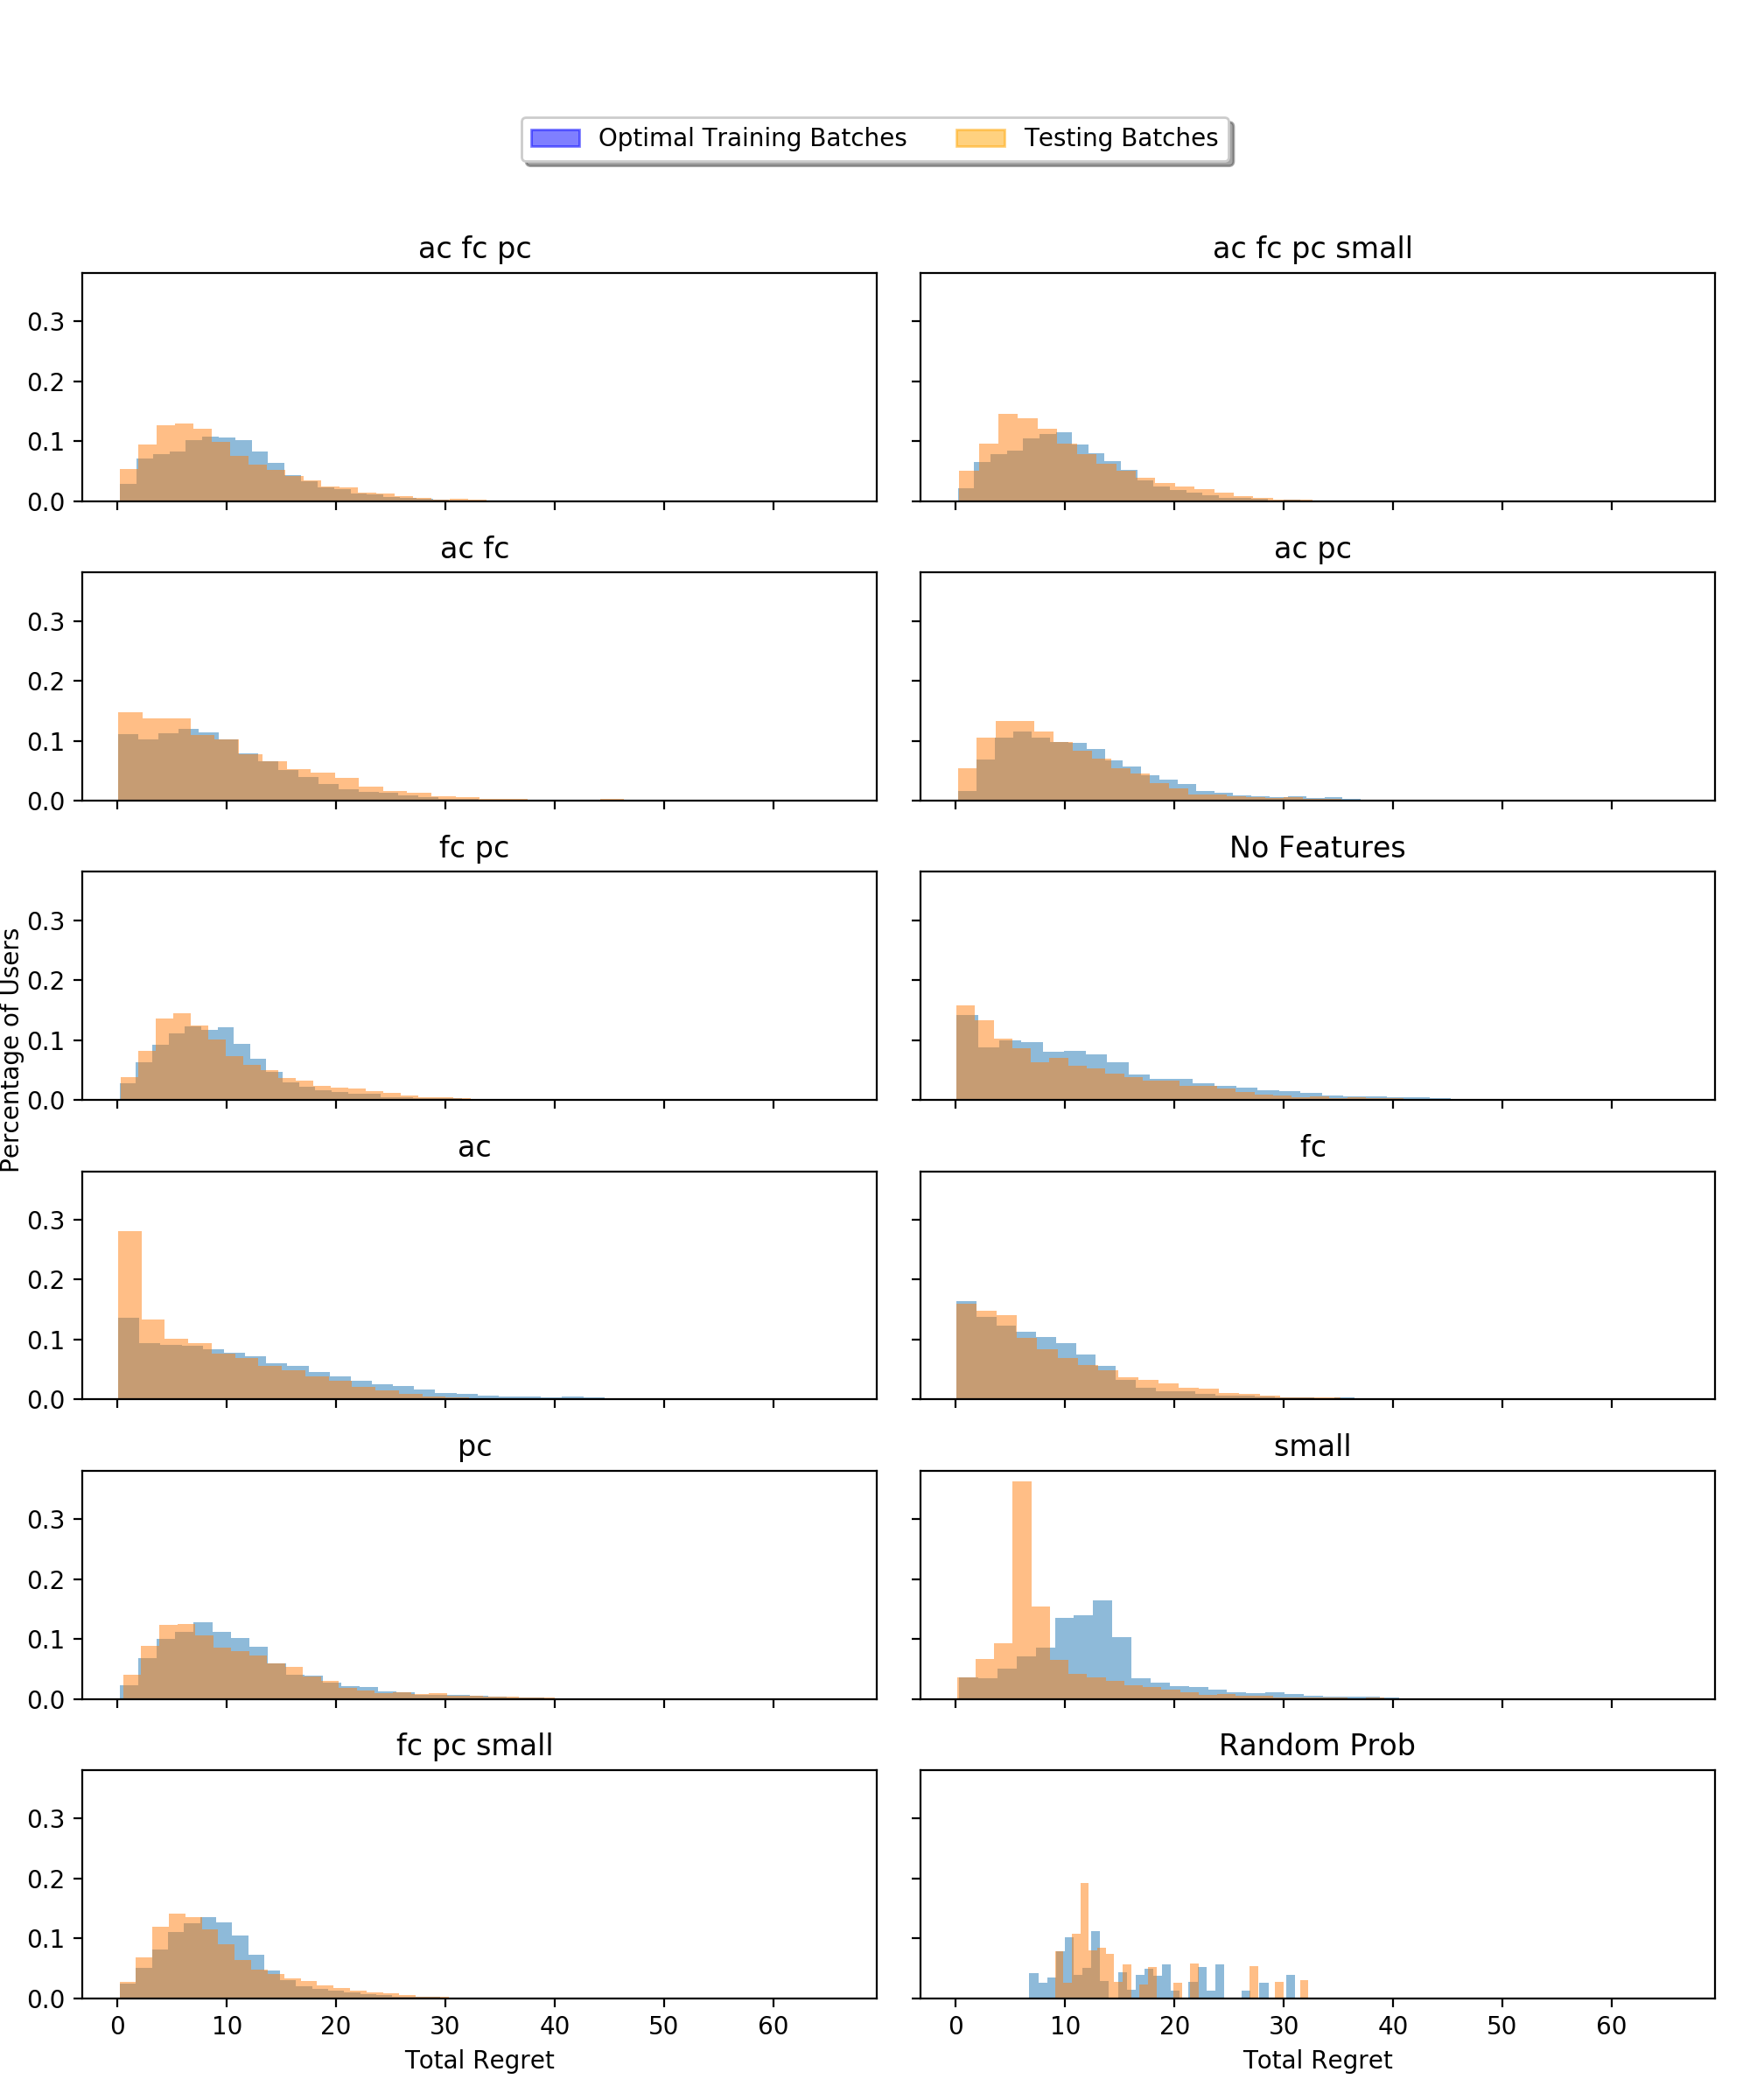
\includegraphics[width=1.35\textwidth,center]{figures/totalregrethists.png}%
\caption{Histogram of all users' total regrets for all Bandit Variants, lower regrets indicate better performance.}
\label{Histogram of all Users' Total Regrets for all Bandit Variants}
\end{figure}

\clearpage

\subsection{$MUER$ Variance Decomposition}
\label{Variance Decomposition}

We study the decompsition of the Total Variance in simulated $MUER$ into Within-User Variance and Betweeen-User Variance.  As we bootstrapped to obtain simulation users, we can reindex to match each simulation user with the $i$-th trial for real user $n$.  Let $Num(n)$ denote the number of times user $n$ was sampled within our set of simulation users.

As we reindex, we denote that simulation $i$ for user $n$ has $MUER$ as $MUER_{n,i}$.  Then, the mean $MUER$ for user $n$ is computed by averaging all $Num(n)$ simulation trials, which we denote as $\overline{MUER}_{n}$.  Finally, we can denote the overall weighted mean across all users as $\overline{MUER}$, which is computed by weighting each user's mean MUER by $Num(n)$.  Recalling that $N = 37$ is the number of real users from the original HeartSteps v1 study while $2500$ is the number of bootstrapped simulation users, we summarize our decompsitions as such:

\begin{align}
\sigma^2_{total} &= \sigma^2_{within} + \sigma^2_{between} \\
\sigma^2_{total} &:= \frac{1}{2500} \sum_{n=1}^N \sum_{i=1}^{Num(n)} \left(MUER_{n,i} - \overline{MUER}\right)^2 \\
\sigma^2_{within} &:= \frac{1}{2500} \sum_{n=1}^{N} \sigma^2_{within,n} \cdot Num(n) \\
\sigma^2_{within,n} &:= \frac{1}{Num(n)} \sum_{i=1}^{Num(n)} \left(MUER_{n,i} - \overline{MUER}_{n}\right)^2 \\
\sigma^2_{between} &:=  \frac{1}{N} \sum_{n=1}^{N} \left(\overline{MUER}_{n} - \overline{MUER} \right)^2
\end{align}

In table \ref{Variance Decomposition Table}, we report the simulation results; these are also depicted in the boxplots of figure \ref{Boxplots of MUER for all Bandit Variants, sorted by mean MUER}.

  \begin{table}[H]
\centering
\begin{tabular}{llrrr}
\toprule
{} &  Batch &  Total var &  Within var &  Between var \\
\midrule
ac             &   Test &   2.661305 &    1.854323 &     0.806983 \\
No Features    &   Test &   2.804786 &    1.856737 &     0.948049 \\
pc             &   Test &   3.144949 &    2.359168 &     0.785780 \\
small          &   Test &   3.162685 &    2.706956 &     0.455729 \\
fc pc          &   Test &   3.358141 &    2.414217 &     0.943925 \\
ac fc          &   Test &   3.382839 &    1.980111 &     1.402729 \\
ac fc pc       &   Test &   3.385391 &    2.016630 &     1.368761 \\
fc             &   Test &   3.407053 &    2.486476 &     0.920577 \\
ac fc pc small &   Test &   3.504155 &    2.074450 &     1.429705 \\
ac pc          &   Test &   6.071459 &    0.486644 &     5.584816 \\
No Features    &  Train &   2.523148 &    1.848379 &     0.674769 \\
ac fc          &  Train &   2.592400 &    1.728600 &     0.863799 \\
ac fc pc       &  Train &   3.062984 &    2.010644 &     1.052340 \\
fc             &  Train &   3.088712 &    2.424037 &     0.664676 \\
small          &  Train &   3.097342 &    2.599052 &     0.498290 \\
fc pc          &  Train &   3.123756 &    2.280590 &     0.843166 \\
ac fc pc small &  Train &   3.222406 &    1.889396 &     1.333010 \\
ac             &  Train &   3.239059 &    2.276554 &     0.962505 \\
pc             &  Train &   3.334281 &    2.360475 &     0.973806 \\
ac pc          &  Train &   3.719548 &    0.524511 &     3.195038 \\
\bottomrule
\end{tabular}
\caption{Variance decomposition into Within-User and Between-User Variance, averaged across $k = 3$ split batches.}
\label{Variance Decomposition Table}
\end{table}

\clearpage

\subsection{Action Centering}

The presence of action centering does not greatly affect many quality metrics.  The $MUER$ variance slightly increases with the presence of this feature.

One observation is found in \ref{QM11train}, we see that the naked variant and the variant with just action centering differ in the fact that the $95\%$ and $75\%$ percentiles for the $\Theta$ MSE is markedly smaller.  In particular, we observe that this does not happen with adding just one of any of the other features, suggesting that lone action centering does well to mitigate poor training as compared to the others.  However, this benefit is highly dampened when comparing the full variant with and without action centering.


\subsection{Feedback Controller}

The addition of a feedback controller slightly decreased the mean $MUER$ as well as the variance.  Looking at histogram \ref{Histogram of all Users' Total Regrets for all Bandit Variants}, the full variant without a feedback controller yields a heavier and longer tail versus with a feedback controller, especially for the testing batches.

While the training $MUER$ remained similar when a feedback controller was added to the naked variant, the testing $MUER$ markedly increased, suggesting that this may not be a good feature to use by itself.

\subsection{Probability Clipping}

Without probability clipping, we note that negative regret is easily achievable -- this is because we keep the regret function as the same $MUER$ that is computed by choosing the optimal of $\pi_\text{min}$ or $\pi_\text{max}$, as to be able to compare different models under the same metrics.

The mean $MUER$ does not change too much and in fact, decreases slightly, but we especially see that the variance and the difference between the $95\%$ and $5\%$ percentiles increase far more over time. 

In practice, it does not seem that there are $MUER$ performance-based reasons to remove the probability clipping, especially with its behavioral and inferential benefits.  Nonetheless, future work may investigate varying levels of probability clipping to infer.

\subsection{Small Contexts}

Removing contextual features from the Full set to the Small set did not yield a large change in training batches, and while the performance between the Small and Full sets in testing batches 1 and 2 are similar, there are particular users in testing batch 3 that yielded a marked increase in the overall regret levels.

This result is surprising -- we may expect that if a smaller set of contextual features would have similar training performance as a larger set, that it would be less prone to overfitting, and have better testing performance.  This suggests that we require the full set of proposed features to maintain regret levels, not due to an overall diminishing of performance, but rather performance on several individuals.

The Small set also slightly pushes the generated probabilities $\pi_{(t,d)}$ downward.



\section{Impact of Tuning Parameters}

In appendix \ref{MUER Minimization Parameter Optimization}, we depict the result of optimizing the full model (ac fc pc) on the first training batch, running through each of the $6$ parameters in order of \\
\noindent $\mathtt{N\_c\_mult},\mathtt{T\_c},\mathtt{sig2\_mult},\mathtt{gamma},\mathtt{lamb},\mathtt{prior\_cov\_mult}$ and cycling through $r_{\text{cycles}} = 4$ times.  The following results observationally hold through the other batches.  



\subsection{$\mathtt{N\_c\_mult}$}

Over the parameter cycling, $\mathtt{N\_c\_mult}$ starts off fairly bumpy, owing to the fact that they only affect quantized values of $N_c$.  While there are strong correspondences between $\mathtt{N\_c\_mult}$ and the average and StdDev $MUER$, the correspondences are not consistent. Higher values of $N_c$ correspond with a less prevalent feedback controller, and correspond with lower $MUER$, but also correspond with a convex StdDev $MUER$ that can either be increasing or decreasing.

The largest effect on mean ranges between a $30\%$ and $40\%$ decrease between suboptimal and optimal values, while the effect on StdDev can be as much as a $60\%$ decrease.

\subsection{$\mathtt{T\_c}$}

Here, we see that $T_c$ is also fairly quantized, and in general does not impact the mean nor standard deviation of the $MUER$ heavily.  Most of the time, there is a slight tendency toward decreased mean $MUER$ but increased StdDev $MUER$ as $T_c$ increases; however, towards the end of the StdDev Cutoff Optimization routine, the impact increases on the Mean $MUER$, and the StdDev $MUER$ actually decreases with $T_c$.

The effects on the mean and StdDev are quite small, both ranging between $1\%-4\%$ as a decrease.

\subsection{$\mathtt{sig2\_mult}$}

In general, we see higher values of $\mathtt{sig2\_mult}$ cause to non-linear decreasing the StdDev $MUER$, and values close to $1$ are chosen.

The effect on the mean is quite small, around $2\%$, while the effect on StdDev can range between $25\% - 40\%$.

\subsection{$\mathtt{gamma}$}

As we tested values of $\gamma \in [0,1]$, we see that the bulk of the effect occurs when $\gamma$ is close to $1$; when $\gamma = 1$ precisely, our Gaussian Process Prior becomes a standard Bayesian normal posterior update.  We see consistently that higher values of $\gamma$ decrease the overall mean $MUER$, but also increase the StdDev $MUER$ significantly.

The effect on mean ranges from $10\% - 25\%$, but the effect on StdDev can range from $400\%-600\%$.

\subsection{$\mathtt{lamb}$}

Seeing as $\lambda$ controls the aggressiveness of the feedback controller once it has been invoked, we expect and observe that tuning its values has a similarly minor effect like with tuning $N_c$ and $T_c$.  Mean and StdDev $MUER$ remain fairly constant, but for values of $\lambda < 0.75$, the effect on the StdDev intensifies, but in a direction dependent on the other parameters.  Notably, because the mean is so constant, it seems we can tune this parameter directly in favor of the StdDev $MUER$.

There is virtually no effect on the mean, except for a $1\%$ fluctuation around $\lambda = 0$, while the effect on StdDev can be from $0\% - 5\%$.

\subsection{$\mathtt{prior\_cov\_mult}$}

For the multiplier on $\Sigma_\Theta = \mathbb{I}$, we see that it does not majorly impact the mean nor StdDev $MUER$ -- however, lower values of the multiplier consistently decreases the mean $MUER$ while increasing the StdDev $MUER$.

While the effect on the mean is about $1\%$ and fairly constant the effect on StdDev $MUER$ is between $5\% - 10\%$ and always decreasing.



  \begin{table}[!h]
	  \centering
\begin{tabular}{|l|rr|}
\toprule
{} &  MUER Min &  StdDev Cutoff \\
\midrule
N\_c\_mult       &     0.777 &          0.526 \\
T\_c            &    67.000 &         70.000 \\
sig2\_mult      &     1.111 &          0.191 \\
gamma          &     1.000 &          0.736 \\
lamb           &     0.349 &          0.100 \\
prior\_cov\_mult &     0.100 &          0.519 \\
\midrule
Train Mean     &     0.062 &          0.072 \\
Train StdDev   &     0.032 &          0.007 \\
Test Mean      &     0.080 &          0.080 \\
Test StdDev    &     0.009 &          0.009 \\
\bottomrule
\end{tabular}
\caption{Optimally tuned parameter values and performance comparisons between Optimization Routines}
\end{table}


% MOVE THIS PART
% Recall that the Signal-to-Noise-Ratio (SNR) is computed as 
% \begin{equation}
% \label{SNR equation}
% 	\frac{\Var(\mathcal{R})}{\sigma^2} = \frac{\Var\left(\begin{bmatrix}
% f_1(\mathcal{S}) \\ A \odot f_2(\mathcal{S})	
% \end{bmatrix}^T\Theta\right)}{\sigma^2}.
% \end{equation}